% Created 2020-09-03 Thu 21:20
% Intended LaTeX compiler: pdflatex
\documentclass[11pt]{article}
\usepackage[utf8]{inputenc}
\usepackage[T1]{fontenc}
\usepackage{graphicx}
\usepackage{grffile}
\usepackage{longtable}
\usepackage{wrapfig}
\usepackage{rotating}
\usepackage[normalem]{ulem}
\usepackage{amsmath}
\usepackage{textcomp}
\usepackage{amssymb}
\usepackage{capt-of}
\usepackage{hyperref}
\usepackage[margin=0.5in]{geometry}
\author{by Michael Barrett}
\date{September 4, 2020}
\title{Object Detection Using HSV Color Detection In OpenCV}
\hypersetup{
 pdfauthor={by Michael Barrett},
 pdftitle={Object Detection Using HSV Color Detection In OpenCV},
 pdfkeywords={},
 pdfsubject={},
 pdfcreator={Emacs 26.3 (Org mode 9.1.9)}, 
 pdflang={English}}
\begin{document}

\maketitle

\section{Overview}
\label{sec:org2923cbe}
The Object Detector detects objects in a photo by color and returns their coordinates in the photo as well as size, shape, and other properties. Currently, objects colored red, blue, and green are detectable. OpenCV's contour detection requires no machine learning making this a fast solution to the problem of detecting objects on a manufacturing table. For HSV color encoding, the level of light or shadow on the object is less important than it would be for color detection with RGB color encoding, allowing an object to be reliably detected as long as it is colored distinctly.
\section{Functionality}
\label{sec:orgd7c4eaf}
\subsection{Detecting a red object}
\label{sec:org274af1d}
\begin{center}
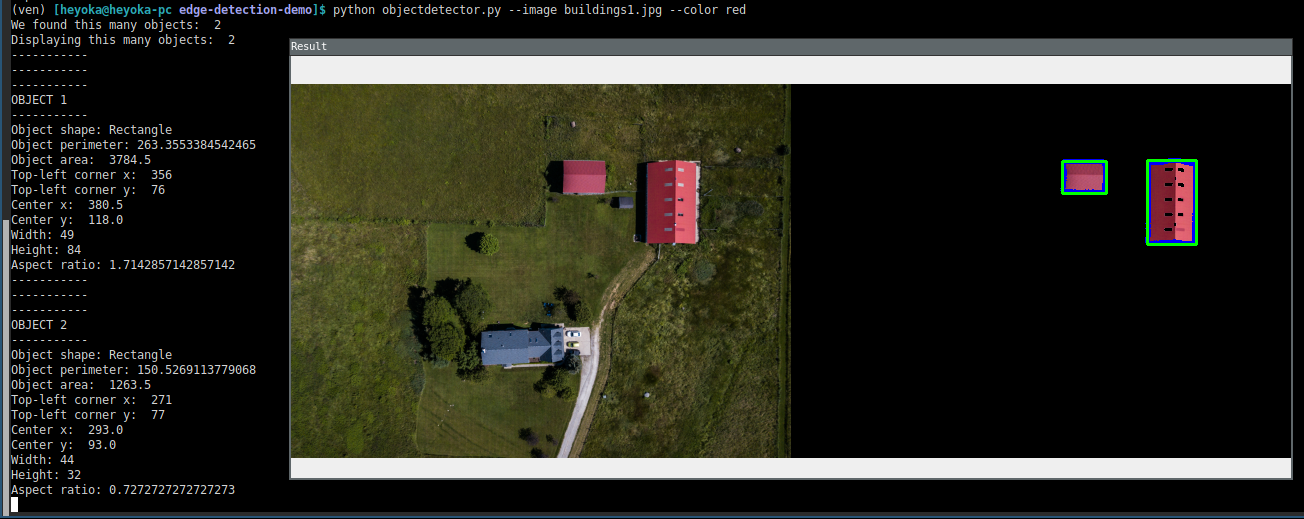
\includegraphics[width=500px]{/home/heyoka/opencv-pix/red-house-detect.png}
\end{center}
\subsection{Detecting a blue object}
\label{sec:org2ce527c}
\begin{center}
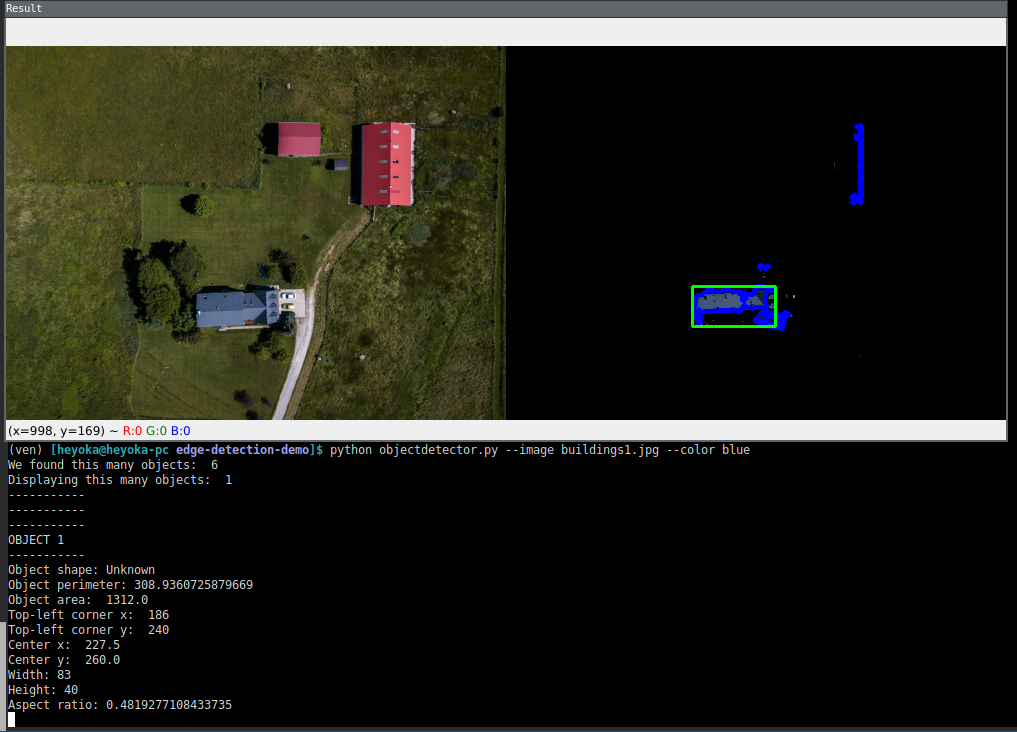
\includegraphics[width=500px]{/home/heyoka/opencv-pix/blue-house-detect.png}
\end{center}
\section{Planned features}
\label{sec:org7cb4f04}
\begin{itemize}
\item The ability to interface with the framework for the manufacturing machines
\item The ability to detect objects with colors other than red, blue, and green
\item The ability to compute the average color of a particular object in the photo as a rudimentary means of object recognition
\item The use of machine learning (custom-trained CNNs) to detect the identity of an object as a finer means of object recognition
\end{itemize}
\end{document}
